% ** Résultats
% *** Sur la base de Réda.
% *** Jolis graphiques.

\section{Results}
\label{sec:results}

The results presented in this section has been obtained on the MNIST
database.  Each sample is encoded as a vector of 784 dimensions
corresponding to a $28 \times 28$ pixels image. Each image represents
a handwritten digit from 0 to 9, defining 9 different classes.
The train dataset is composed of 60000 images and the test dataset of 10000.\\

The classifier used for the benchmark is simply a nearest mean
classifier.  It associates to a sample the class that minimizes the
square distance between the class mean and
the sample mean.\\

{\bf Note:} Because of memory consumption issues, the HLDA algorithm
is run on smaller dimension samples. To do that, a PCA is applied to
the samples keeping the 250 highest eigenvectors.

The Matlab implementation we use for the HLDA is the one given in \cite{burget.2004}.

\subsection{HLDA parameters}

The HLDA method has a lot of parameters, some are linked to the
dataset and some must be tuned by the user.

\paragraph{Number of meaningful dimensions} The principal parameter to
find is the number of dimension kept by the algorithm, called $p$.

\begin{figure}[H!]
  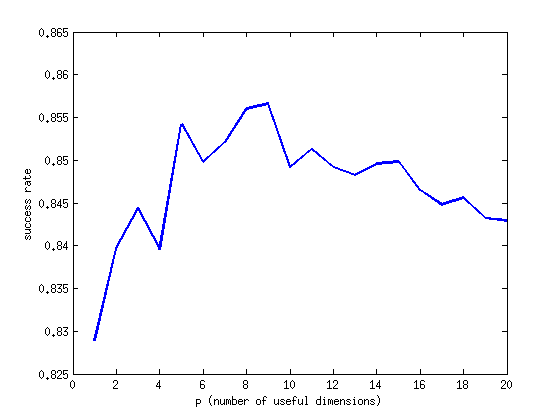
\includegraphics[scale=0.75]{img/bench-classes}
  \caption{Variation of the $p$ parameter}
  \label{img:classes}
\end{figure}

Interestingly, figure \ref{img:classes} shows that the best
classification ratio happens for $p = 9$ which is exactly the number
of dimensions kept by the LDA. Furthermore the farther we get from it
the worst the classification value get.

\paragraph{Convergence problem} The current implementation of the HLDA does not converge toward a better
solution but toward a worst one.

\begin{figure}[H!]
  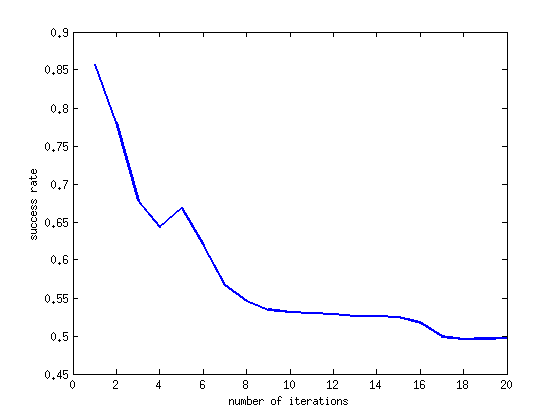
\includegraphics[scale=0.75]{img/bench-iterations}
  \caption{Variation of number of iteration for the numerical approximation}
  \label{img:iter}
\end{figure}

Figure \ref{img:iter} shows that as the number of iterations increase, the classification ratio decrease.

\paragraph{Points separation} To visualize the effect of the tested method on the data-set we present a plot
of the first two coordinates for each samples. In Figure \ref{img:classif} each point has a color corresponding to its
class.

\begin{center}
\begin{figure}[H!]
  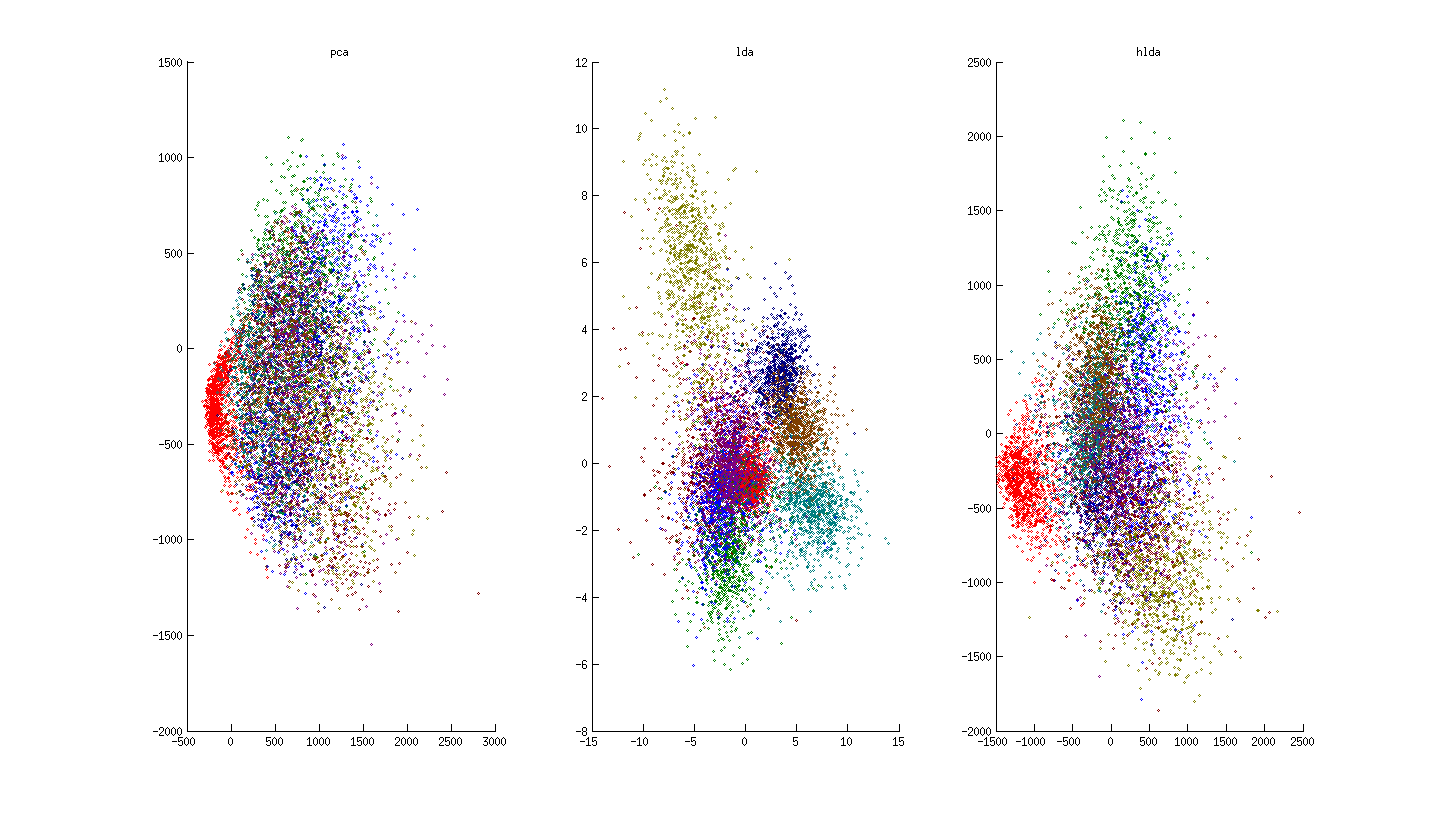
\includegraphics[scale=0.30]{img/classif}
  \caption{Classification results, from left to right: PCA, LDA, HLDA}
  \label{img:classif}
\end{figure}
\end{center}

The PCA as expected shows a very poor separation between classes whereas the LDA and HLDA
methods better separates classes. The results for the HLDA are not as good as expected,
maybe due to implementation issues.
